\chapter{Conclusions and Future Research} \label{conclusions}

In this chapter, conclusions about the dissertation will be drawn and the
author's contributions will be presented. Further work in the future, including
investigation and application of Plasmonic effects in CSNW; heterogeneous
integration of CSNW active and passive components on the silicon-based photonic
integrated circuit, will be discussed.

\section{Summary of Contributions}

As mentioned previously, communication of information, together with storage
and computation form a “grand challenge” of the information age. Recently, the
analysis of big data has become the engine for societal, financial, scientific,
and technological endeavors. This demands an infrastructure that is capable of
fast and reliable high volume data processing. Traditionally, this requirement
was fulfilled by silicon technology. However, silicon-based technology has its
own limitations, such as speed limit and heat dissipation problem. In order to
process high volume data, we need data computation, storage and communication
work as three fundamental functions of a computation cell. And core-shell
nanowires will play an important role in this regime with their extraordinary
optical properties.

In conclusion, fabrication techniques, electrical and optical properties of
core-shell nanowires grown on GaAs or Si substrates were discussed here
emphasizing the analysis of resonant optical modes which depend both radially
and axially on the geometries of the nanowires. This shows how such
sub-wavelength structures can form optical cavities as-grown, without needing
sophisticated facet mirrors. In addition, we show how the fortuitous overlap of
the reduced dimensional electronic wave functions and the photonic modes is
responsible for the extraordinary optoelectronic properties of core-shell
nanowires. Such nano-structures have been developed on heterogeneous
substrates, particularly silicon, and as such becoming an important component
in the next generation of photonic integrated circuits which are particularly
useful in meeting the grand challenge of low energy and fast speed computation.

In this dissertation, we designed and fabricated the CSNWs based
heterostructure devices, measured and simulated their opto-electronic
properties, and compared it with bulk structures. The static behavior
simulations, including 2-D potential profile, electric field distributions, and
carrier concentration, were performed with commercially available software. The
light confinement and distribution in the CSNWs was investigated by FDTD
simulation. The simulation revealed the transverse and longitudinal plane waves
in the resonance frequency enhanced the optical confinement of these sub-micron
scale cavities.

We showed that how low dimensional electron density distribution change the
optical transition rates when a small perturbation is introduced by light which
results in large enhancement of optical properties.

In addition, we designed a CSNW based laser and modeled its static and dynamic
lasing behavior by calculating the optical gain and threshold current density,
demonstrated that how reduced dimensional electron states enhance the overall
gain and emission efficiency compared to its bulk counterpart.

The major contributions of this thesis are (1) design, fabricate and
characterize the hexagonal CSNWs grown on Si or GaAs substrates, revealing
enhanced optical properties, such as absorption, emission and lasing; (2)
simulation and analysis of light confinement and propagation mechanism in
CSNWs; (3) simulation and analysis of electron distribution in the hexagonal
CSNWs; (4) derived dimensional dependent band-to-band transition rates and
proposed the spacial overlapping of the confined light with reduced electronic
wave function greatly enhanced the optical transition rates; (5) modeled and
calculated the optical gain and output power in order to justify that lower
dimensional electron states will facilitate the lasing behaviors of CSNW based
laser and produced more light compare to their bulk counterparts.

\section{Outline of the future work}

Several aspects of research, such as in-depth theoretical work, wide ranges of
applications, further material explorations, can be extended from the present
work in the future as both breadth and depth are concerned. These issues
include collective behavior in low dimensional structures, optimization of
growth techniques and materials, development of Schottky contacts and
exploiting electrical injection applications, employment of plasmonic effects,
heterogeneous integration on Silicon based photonic integrated circuits.

\subsection{Plasmonic Effects}

Low dimensional electron gases exist at the heterointerfaces of core-shell
nanowires (CSNWs). For example, the GaAs/AlGaAs CSNWs typically form a
hexagonal structure in which six (6) pillars of 1D charge at the vortices, and
six (6) sheets of 2D charge at facets are formed~\cite{Wang:2015hz}. At the
same time, nanowires (NW) have also been shown to be capable of confining light
in their sub-wavelength nano-structure, supporting photonic modes, and
producing resonant cavities without the need for polished end facets. We have
previously shown how the electronic wave functions that are thus formed affect
the optical transition rates, resulting in orders of magnitude  enhancement in
absorption and emission of light. Here we propose the plasmonic effects of the
confined charge on the optical properties of CSNWs.

The finite difference time domain (FDTD) simulations identify the
surface plasmon resonance modes which affect light confinement in hexagonal
CSNWs, and help form a high quality factor resonant cavity. We
compare regular CSNW, with a) wires covered with metal which produces surface
plasmon-polaritons (SPP’); b) NWs covered with metal that is sandwiched between
the core and the outer, shell; and c) two-dimensional electron gas (2DEG)
which embedded at the heterointerace of CSNWs. Results show that the 2DEG
behaves similarly to an embedded metallic surface, allowing for highly
localized light confinement in these wires without the need for vertical
structures such as Bragg mirrors commonly used in vertical cavity surface
emitting lasers (VCSEL’s). Besides affecting the cavity, the 2DEG enhances  the
transition rates due to the plasmon-electron interaction, facilitating not only
photonic stimulated emission and lasing, but also  surface plasmon
amplification by stimulated emission of radiation~\cite{Bergman:2003vo}.

The electromagnetic wave traveling of the Surface Plamon Polariton (SPP)
involves both charge motion in electron reservoir (e.g., metal, graphene and
2DEG) and waves in the dielectric or air. Instead of using any metallic
materials, Core-Shell nanowires (CSNWs) can naturally form two-dimensional
electron gas (2DEG) at the heterojunction interface and even large
one-dimensional pillar of charge at the corners of thier hexagonal facets.

\begin{figure}
  \caption[An FDTD-simulated electric field profile of (a) a hexagonal core-shell nanowire (CSNW), (b) CSNW covered with silver coating, (c) CSNW with embeded silver layer between the core and the shell, (d) CSNW with embedded 2DEG.]{An FDTD-simulated electric field profile (linear scale) of (a) a hexagonal core-shell nanowire (CSNW), (b) photonic modes are affected by plamonic modes in a CSNW covered with silver coating, (c) CSNW with embedded silver layer between the core and the shell; (d) plasmonic and photonic modes of CSNW with embedded 2DEG show similar effects compared to embedded metal. The black boundaries represent the interface betweeen layers of the structure.}
  \centering
  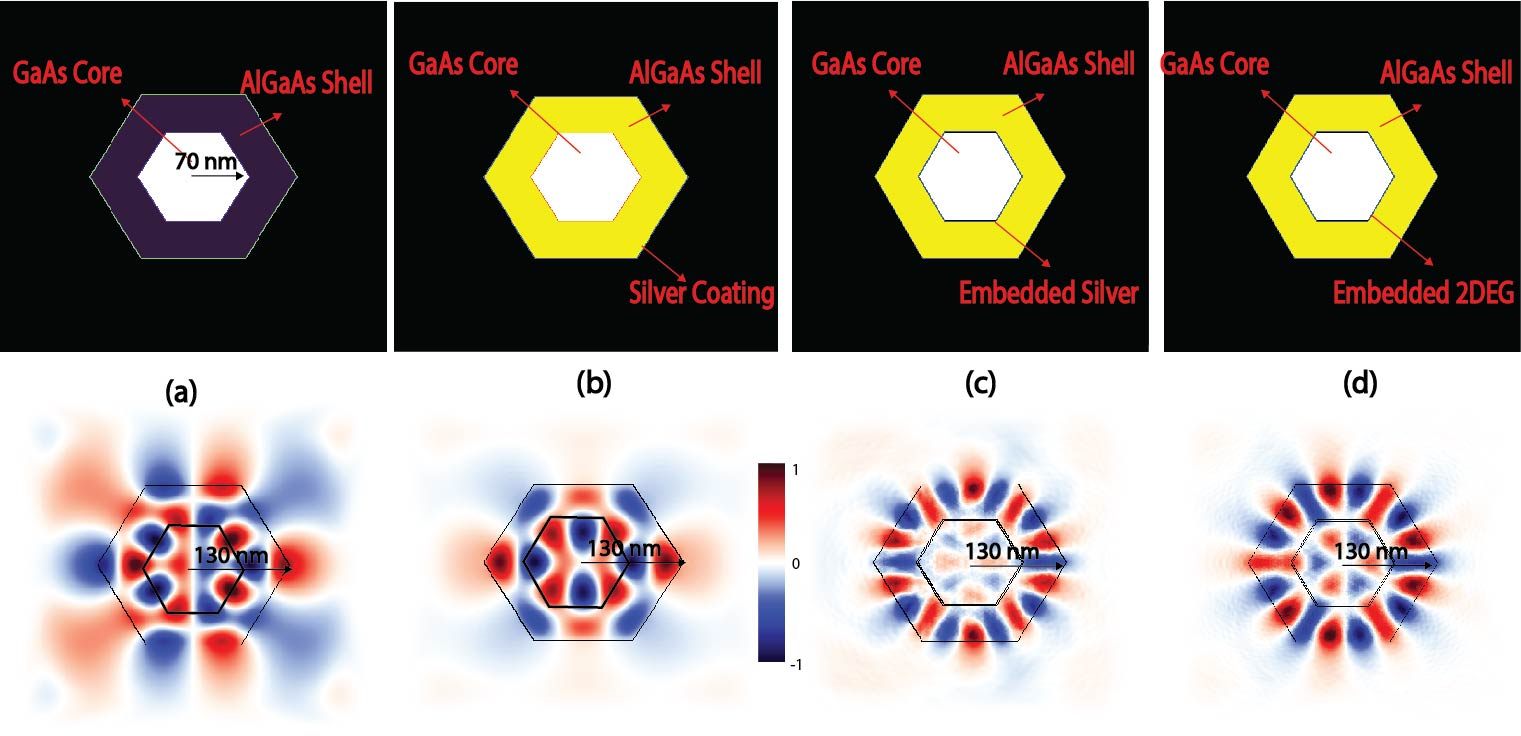
\includegraphics[width=\textwidth]{pictures/Conclusion/PlasmonMode}
  \label{PlasmonMode}
\end{figure}

Figure~\ref{PlasmonMode} shows the FDTD-simulated electric field profile
(linear scale) in the transverse plane of (a) CSNW; (b) CSNW with silver
coating; (c) CSNW with and embedded silver layer between the core and the
shell; (d) CSNW with 2DEG at the hetero-interface. As shown in
Fig~\ref{PlasmonMode}, coating the wire with metal introduces plasmonic modes
in the structure that enhance light confinement. Metal embedded between the
core and the shell has similar effect. Importantly, we observe that similar
plasmonic features can be obtained due to the 2DEG that is embedded in
CSNW~\cite{montazeri2016plasmonic}.

\subsection{Heterogeneous Integration on PIC}

Recently, the increasing demand for high-speed low-power computation and
communication has driven the growth of photonics integrated circuit (PIC)
technology with projected market size of a billion dollars by 2018. Silicon
photonics have received significant attention as it benefits from
well-established complementary metal-oxide-semiconductor (CMOS) technology.
Lack of an efficient silicon-based light source and photodetector, has
motivated development of technologies for heterogeneous integration of
efficient III-V semiconductor light sources and detector with silicon chips.
Here we present core-shell nanowires (CSNWs) as versatile low-dimensional
optoelectronic systems as a replacement to their conventional thin film
counterparts in heterogeneous integration in silicon photonics. These CSNWs
have extraordinary performance in light generation, absorption, light
modulation, energy generation, and high-speed optical detection. Finally, we
elaborate on a vision for a low-cost high-performance silicon photonics chip
based on a core-shell nanowire platform. In this scheme, CSNWs are applied as
high-speed low-power optical detectors, light source, and waveguides.

In order to process high volume data, we need data computation, storage, and
communication to work in concert as the three fundamental functions of a
computation cell. As schematically shown in Fig.~\ref{NWPIC_NB}, a monolithic
nanosystem may be envisioned, which incorporates NWs as waveguides, detectors,
photovoltaic cells, antennas, modulators, (photo)capacitors, LEDs and lasers.
These components may be incorporated in circuit layers, such as
network-on-chip. Different layers can communicate using NW through-silicon vias
(TSVs). Similar low-power/high-performance advantags can be realized through
achievement of high interconnect densities on the 2.5D through-Si-interposer
(TSI) as reported in reference~\cite{Zhang:2015ec} 

Performance enhancement of CSNWs can be attributed to the formation of confined
quasi-one-dimensional electron gas at the vortices, and two-dimensional
electron gas at the facets of the hexagonally shaped GaAs/AlGaAs core-shell
hetero-interface.  These reduced dimensional confined charge plasma affect
optical transition rates, facilitate population inversion, and collect
optically generated electrons and wholes before they transit to the contacts.
Additionally these plasmons, which are unique to CSNWs, affect waveguiding and
optical cavity properties of CSNWs and can be used as waveguides, modulators
and photocapacitors.

The proposed integrated photonic platform is schematically depicted at the
bottom part of Fig.~\ref{NWPIC_NB} with multiple key components implemented
through utilizing core-shell nanowires. This monolithic nanosystem incorporates
CSNWs as waveguides, detectors, photovoltaic cells, antennas, modulators, LEDs,
and lasers. These components may be incorporated in circuit layers, such as
networks on chip. Additionally, they can be used for 3D integration using NW
through-silicon vias (TSVs). Such a circuit may compete with manufacturing
methods such as flip-chip bonding and achieves further miniaturization by
incorporating high-performance nanowires in vertical architectures to replace
large surface area thin film structures such as vertical cavity surface
emitting lasers (VCSELs).

In conclusion, CSNW demonstrate unique combination of plasmonic, photonic, and
electronic properties which makes them versatile high-performance
optoelectronic devices including Lasers, LEDs, photodetectors, solar cells,
waveguides, and optical amplifiers. Since they can be grown from a wide range
of material including GaAs, InP, and GaN, at different directions and on
foreign substrates such as oxides, Graphene, Si, and III-Vs, they offer a
competitive platform for photonic integrated circuits, and specifically for
heterogeneous integration in silicon photonics chips,
photodetectors/photocapacitors, antennas and waveguides.

\begin{figure}
  \caption{Schematic depiction of an optoelectronic nanosystem may include key components such as NW LED/laser source, photodetector/photocapacitor, NW antennas, and NW-enabled network-on-chip integrated on silicon.}
  \centering
  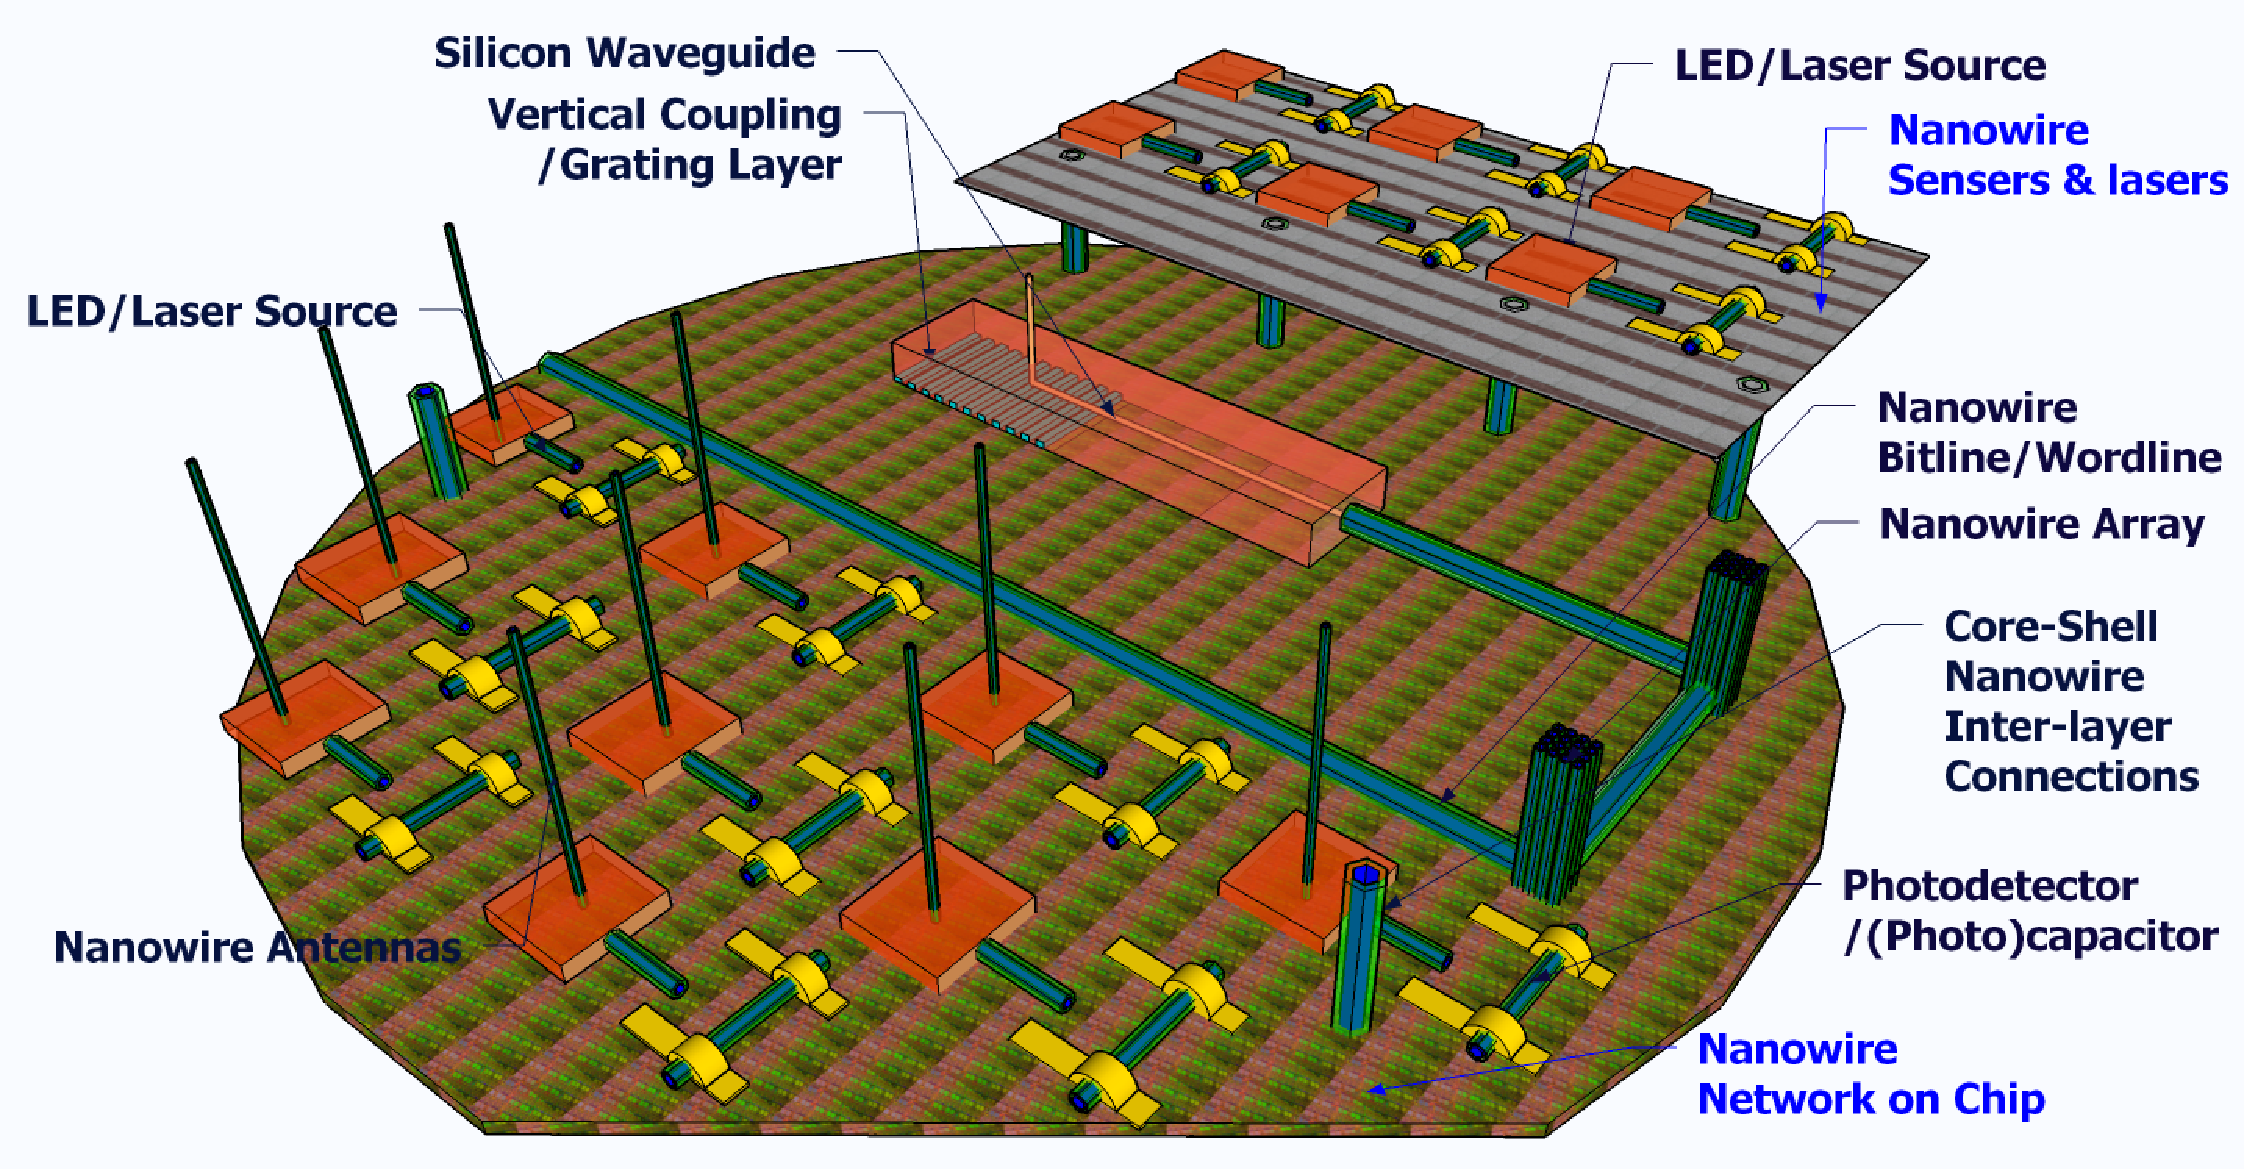
\includegraphics[width=\textwidth]{pictures/Conclusion/NWPIC_NB}
  \label{NWPIC_NB}
\end{figure}
